\documentclass[12pt,a4paper]{article}

% ── Packages ─────────────────────────────────────────────────
\usepackage[utf8]{inputenc}
\usepackage[T1]{fontenc}
\usepackage{lmodern}
\usepackage{geometry}
\usepackage{xcolor}
\usepackage{fancyhdr}
\usepackage{listings}
\usepackage{amsmath,amssymb}
\usepackage{graphicx}
\usepackage{booktabs}
\usepackage{tabularx}
\usepackage{parskip}
\usepackage{eso-pic}
\usepackage{hyperref}
\usepackage{float}
\usepackage{caption}
\usepackage{array}

% ── Page Geometry ──────────────────────────────────────────
\geometry{left=2.5cm, right=2.5cm, top=2.8cm, bottom=2.8cm, headheight=14pt}

% ── Colour Palette ─────────────────────────────────────────
\definecolor{primaryblue}{RGB}{0,51,102}
\definecolor{accentblue}{RGB}{0,102,153}
\definecolor{codebg}{RGB}{248,248,248}
\definecolor{codeframe}{RGB}{200,200,200}
\definecolor{darkgreen}{RGB}{0,120,60}
\definecolor{darkred}{RGB}{160,30,30}

% ── Custom Box Environments ────────────────────────────────
\newenvironment{foplbox}%
  {\vspace{6pt}\par\noindent{\color{accentblue}\hrule height 1pt}\vspace{4pt}\noindent\ignorespaces}%
  {\par\nopagebreak\noindent{\color{accentblue}\hrule height 1pt}\vspace{8pt}}

\newenvironment{tracebox}%
  {\vspace{6pt}\par\noindent{\color{darkgreen}\hrule height 0.8pt}\vspace{2pt}%
   \begin{quote}\small\ignorespaces}%
  {\end{quote}\nopagebreak\noindent{\color{darkgreen}\hrule height 0.8pt}\vspace{6pt}}

% ── Listings Style: Prolog ─────────────────────────────────
\lstdefinestyle{prolog}{%
  language=Prolog,
  basicstyle=\ttfamily\small,
  keywordstyle=\color{primaryblue}\bfseries,
  commentstyle=\color{gray}\itshape,
  stringstyle=\color{darkred},
  numberstyle=\tiny\color{gray},
  numbers=left, numbersep=6pt,
  frame=none,
  breaklines=true, showstringspaces=false,
  tabsize=2, captionpos=b,
  xleftmargin=18pt,
  aboveskip=10pt, belowskip=6pt
}

% ── Listings Style: Python ─────────────────────────────────
\lstdefinestyle{python}{%
  language=Python,
  basicstyle=\ttfamily\small,
  keywordstyle=\color{primaryblue}\bfseries,
  commentstyle=\color{gray}\itshape,
  stringstyle=\color{darkred},
  numberstyle=\tiny\color{gray},
  numbers=left, numbersep=6pt,
  frame=none,
  breaklines=true, showstringspaces=false,
  tabsize=2, captionpos=b,
  morekeywords={True,False,None},
  xleftmargin=18pt,
  aboveskip=10pt, belowskip=6pt
}

% ── Listings Style: Output ─────────────────────────────────
\lstdefinestyle{output}{%
  basicstyle=\ttfamily\small,
  frame=none,
  breaklines=true, captionpos=b,
  xleftmargin=18pt,
  aboveskip=8pt, belowskip=4pt
}

% ── Section Formatting ─────────────────────────────────────
\makeatletter
\renewcommand{\section}{\@startsection{section}{1}{\z@}%
  {-3.0ex \@plus -1ex \@minus -.2ex}%
  {1.5ex \@plus.2ex}%
  {\normalfont\Large\bfseries\color{primaryblue}}}
\renewcommand{\subsection}{\@startsection{subsection}{2}{\z@}%
  {-2.5ex\@plus -1ex \@minus -.2ex}%
  {1.0ex \@plus .2ex}%
  {\normalfont\large\bfseries\color{accentblue}}}
\renewcommand{\subsubsection}{\@startsection{subsubsection}{3}{\z@}%
  {-2.0ex\@plus -1ex \@minus -.2ex}%
  {0.8ex \@plus .2ex}%
  {\normalfont\normalsize\bfseries\color{accentblue!80!black}}}
\makeatother

% ── Header / Footer ────────────────────────────────────────
\pagestyle{fancy}
\fancyhf{}
\fancyhead[L]{\small\textit{Lab Report --- Machine Learning Pipeline on the Iris Dataset}}
\fancyhead[R]{\small\textit{Nabina Thapa (080BCT047)}}
\fancyfoot[C]{\thepage}
\renewcommand{\headrulewidth}{0.4pt}
\renewcommand{\footrulewidth}{0.4pt}

% ── Hyperref Setup ─────────────────────────────────────────
\hypersetup{colorlinks=true, linkcolor=black, urlcolor=black}

\begin{document}

% ═══════════════════════════════════════════════════════════
%  COVER PAGE (bordered, plain style)
% ═══════════════════════════════════════════════════════════
\thispagestyle{empty}
\AddToShipoutPictureBG*{%
  \AtPageLowerLeft{%
    \hspace{1.2cm}\raisebox{1.2cm}{%
      \color{black}\framebox[\dimexpr\paperwidth-2.4cm\relax]{%
        \rule{0pt}{\dimexpr\paperheight-2.4cm\relax}}%
    }%
  }%
}

\begin{center}

\vspace*{1.4cm}

\includegraphics[width=0.22\textwidth]{emblem.png}\\[0.6cm]

{\Large TRIBHUVAN UNIVERSITY}\\[0.35cm]
{\large INSTITUTE OF ENGINEERING}\\[0.15cm]
{\large PULCHOWK CAMPUS}\\[1.4cm]

{\bfseries\large A LAB REPORT\\
ON\\[0.2cm]
Machine Learning Pipeline: Generative vs. Discriminative Models,\\
Model Capacity, and Cross-Entropy on the Iris Dataset}

\vspace{2.2cm}

{\rule{0.3pt}{2.3cm}}\hspace{1.4cm}{\rule{0.3pt}{2.3cm}}\hspace{1.4cm}{\rule{0.3pt}{2.3cm}}

\vspace{2.6cm}

\end{center}

\begin{flushleft}
\underline{\textbf{SUBMITTED BY:}}\\[0.4cm]
Name: Nabina Thapa\\[0.2cm]
Roll No.: 080BCT047\\[0.2cm]
Lab No.: 08
\end{flushleft}

\vspace{-1.9cm}
\begin{flushright}
\underline{\textbf{SUBMITTED TO:}}\\[0.4cm]
Department of Electronics\\[0.2cm]
and Computer Engineering
\end{flushright}

\vfill
\clearpage
% \ClearShipoutPictureBG
\setcounter{page}{1}

% ═══════════════════════════════════════════════════════════
%  TABLE OF CONTENTS
% ═══════════════════════════════════════════════════════════
\tableofcontents
\newpage

% ═══════════════════════════════════════════════════════════
\section{Objectives}

\begin{enumerate}
  \item To build a complete \textbf{machine learning pipeline} on the Iris dataset, with stratified training, validation, and test splits.
  \item To train and fairly compare a \textbf{generative model} (Gaussian Naive Bayes) and a \textbf{discriminative model} (Logistic Regression) on the same data.
  \item To study \textbf{model capacity} using Decision Trees of varying depth, and to identify settings that underfit and settings that overfit.
  \item To select a hyperparameter using validation data only, and to report an honest, single evaluation on the held-out test set.
  \item To compute \textbf{cross-entropy} (log loss) for a probabilistic classifier and relate it to the ideas of \textbf{MLE and MAP} estimation.
\end{enumerate}

% ═══════════════════════════════════════════════════════════
\section{Theory}

A supervised learning pipeline consists of preparing data, choosing a model, training it, validating it, and finally evaluating it once on unseen data. The Iris dataset (150 samples, 4 numerical features, 3 classes) is small and clean, which makes it convenient for studying these steps directly rather than being distracted by data-cleaning issues.

\subsection{Generative vs. Discriminative Models}

A \textbf{generative} model, such as Gaussian Naive Bayes, learns the class-conditional distribution $p(x \mid y)$ for each class and uses Bayes' rule to obtain $p(y \mid x)$. A \textbf{discriminative} model, such as Logistic Regression, models $p(y \mid x)$ directly, without describing how the input itself was generated.

\subsection{Model Capacity, Bias and Variance}

\textbf{Model capacity} describes how flexible a model is. A model with too little capacity cannot represent the true decision boundary and \textbf{underfits} -- it performs poorly on both the training and validation data. A model with too much capacity can memorize the training data, including its noise, and \textbf{overfits} -- high training accuracy but a noticeably lower validation accuracy. \textbf{Bias} is the systematic error of an overly simple model (underfitting); \textbf{variance} is the sensitivity of a model to the particular training sample it saw (overfitting).

\subsection{Cross-Entropy, MLE and MAP}

For a predicted probability $\hat p_y$ assigned to the true class $y$, the cross-entropy (negative log-likelihood) of a single prediction is
\[
  \mathrm{Cost} = -\log(\hat p_y).
\]
As $\hat p_y \to 1$ the cost goes to $0$; as $\hat p_y \to 0$ the cost diverges, so confidently wrong predictions are penalized heavily. \textbf{Maximum Likelihood Estimation (MLE)} chooses parameters $\theta$ that maximize the likelihood of the observed data, $\theta^{\mathrm{MLE}} = \arg\max_\theta \prod_i p(x^{(i)}\mid\theta)$. \textbf{Maximum A Posteriori (MAP)} estimation additionally multiplies in a prior $p(\theta)$, $\theta^{\mathrm{MAP}} = \arg\max_\theta \prod_i p(x^{(i)}\mid\theta)\,p(\theta)$, which in Logistic Regression corresponds to $L_2$-regularizing the weights towards zero.

% ═══════════════════════════════════════════════════════════
\section{Methodology}

The Iris dataset was loaded with \texttt{scikit-learn} and split exactly as specified in the lab sheet: an $80/20$ stratified split sets aside the test set, and the remaining $80\%$ is split $75/25$ into training and validation sets. All four features were standardized with a \texttt{StandardScaler} fitted only on the training data. Python 3.12 with \texttt{scikit-learn} 1.9, \texttt{pandas} and \texttt{matplotlib} was used throughout; the code was written in a single script and run from the terminal.

% ═══════════════════════════════════════════════════════════
\section{Implementation}

\subsection{Data Preparation and Model Comparison}

The dataset is split and scaled first, after which Gaussian Naive Bayes and Logistic Regression are trained on the same training data and scored on the validation set.

\lstinputlisting[style=python, firstline=46, lastline=90, caption={\texttt{pipeline.py} -- data split and model comparison}]{code/pipeline.py}

\textbf{Command and output:}
\begin{tracebox}
\begin{verbatim}
$ python pipeline.py
split sizes -> {'train': 90, 'val': 30, 'test': 30}
NaiveBayes val acc = 0.933, LogisticRegression val acc = 0.933
\end{verbatim}
\end{tracebox}

\subsection{Decision Tree Capacity and Hyperparameter Selection}

Decision Trees are trained at four depths, the best depth is chosen using validation accuracy, and that single choice is checked once on the test set.

\lstinputlisting[style=python, firstline=96, lastline=144, caption={\texttt{pipeline.py} -- capacity sweep and hyperparameter selection}]{code/pipeline.py}

\textbf{Command and output:}
\begin{tracebox}
\begin{verbatim}
$ python pipeline.py
depth=1    train=0.667  val=0.667
depth=3    train=0.989  val=0.900
depth=5    train=1.000  val=0.933
depth=None train=1.000  val=0.933
chosen depth: 5 -> test accuracy: 0.933
shallow tree (depth=1): 0.6666666666666666 0.6666666666666666
unrestricted tree (depth=None): 1.0 0.9333333333333333
\end{verbatim}
\end{tracebox}

\subsection{Cross-Entropy and MLE/MAP Analysis}

The validation log loss is computed for Logistic Regression, and the most confident correct and most confident wrong predictions are pulled out with \texttt{pandas} for closer inspection. Regularization strength $C$ is then swept to illustrate the MLE/MAP trade-off.

\lstinputlisting[style=python, firstline=150, lastline=212, caption={\texttt{pipeline.py} -- cross-entropy and MLE/MAP sweep}]{code/pipeline.py}

\textbf{Command and output:}
\begin{tracebox}
\begin{verbatim}
$ python pipeline.py
val log loss: 0.21527889101774805
best correct prediction:
 true_label                   0
pred_label                   0
true_class_name         setosa
prob_of_true_class    0.996551
loss                  0.003455
correct                   True
Name: 12, dtype: object
worst wrong prediction:
 true_label                     1
pred_label                     2
true_class_name       versicolor
prob_of_true_class      0.261827
loss                    1.340072
correct                    False
Name: 10, dtype: object
\end{verbatim}
\end{tracebox}

% ═══════════════════════════════════════════════════════════
\section{Results}

\begin{table}[H]
\centering
\caption{Lab 8 result summary}
\begin{tabularx}{\textwidth}{@{}l >{\raggedright\arraybackslash}X >{\raggedright\arraybackslash}X@{}}
\toprule
\textbf{Task} & \textbf{Metric} & \textbf{Value} \\
\midrule
Data split               & train / val / test samples        & 90 / 30 / 30 \\
Generative vs.\ discriminative & validation accuracy (NB / LogReg) & 0.933 / 0.933 (tie) \\
Decision tree capacity   & underfit at depth=1, overfit at depth=None & train 0.667--1.000, val 0.667--0.933 \\
Hyperparameter selection & chosen \texttt{max\_depth} / test accuracy & 5 / 0.933 \\
Cross-entropy            & validation log loss                & 0.215 \\
MLE vs.\ MAP             & validation accuracy across $C \in [10^{-3},10^{3}]$ & 0.800 -- 0.933 \\
\bottomrule
\end{tabularx}
\end{table}

\begin{figure}[H]
\centering
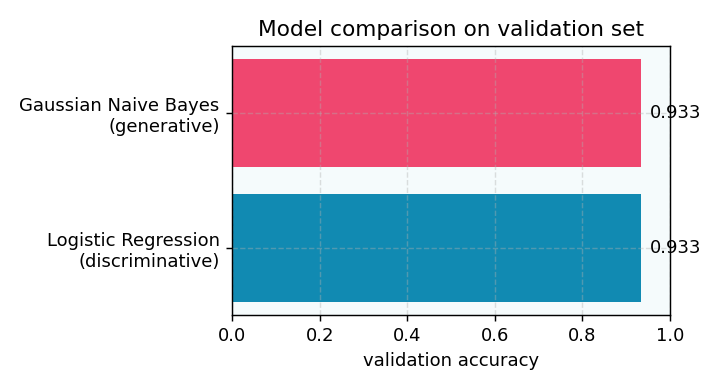
\includegraphics[width=0.6\textwidth]{outputs/gen_vs_disc.png}
\caption{Validation accuracy: Logistic Regression vs. Gaussian Naive Bayes.}
\end{figure}

\begin{figure}[H]
\centering
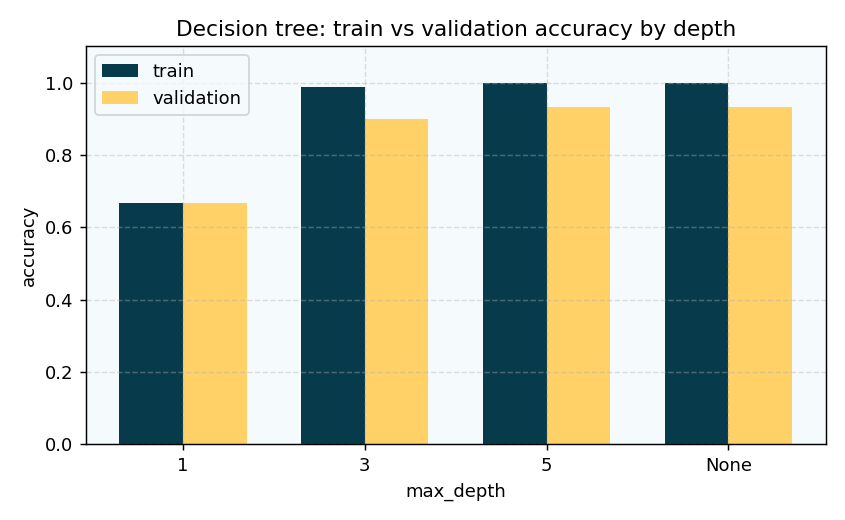
\includegraphics[width=0.7\textwidth]{outputs/tree_capacity.png}
\caption{Training vs. validation accuracy at each Decision Tree depth.}
\end{figure}

\begin{figure}[H]
\centering
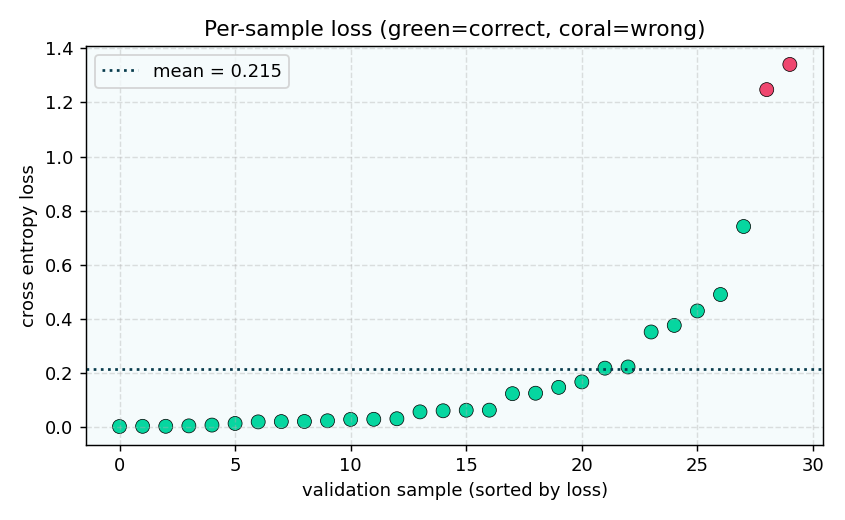
\includegraphics[width=0.7\textwidth]{outputs/cross_entropy.png}
\caption{Per-sample cross-entropy loss on the validation set (green = correct, coral = misclassified).}
\end{figure}

\begin{figure}[H]
\centering
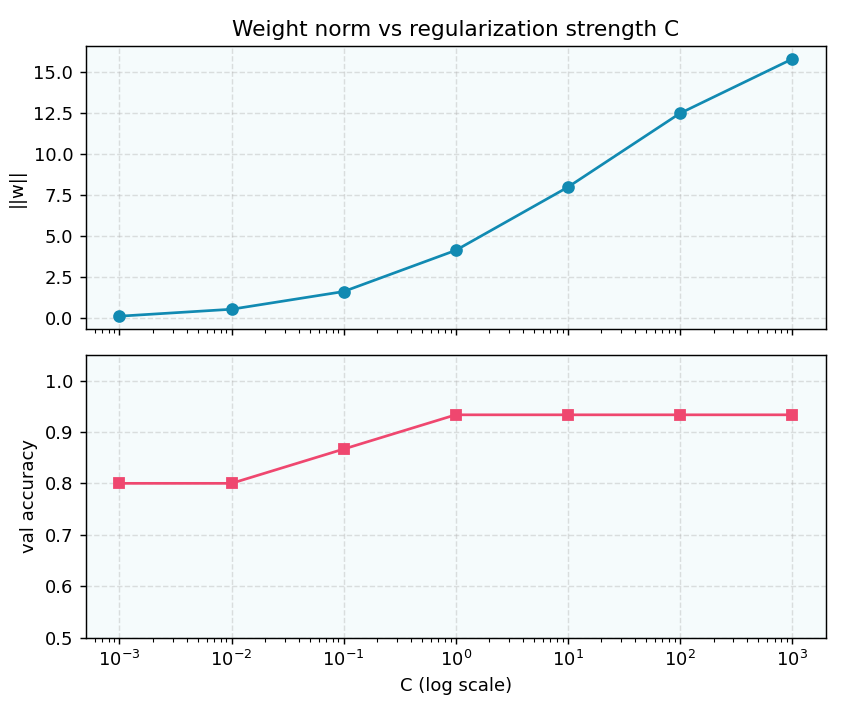
\includegraphics[width=0.7\textwidth]{outputs/mle_map.png}
\caption{Weight norm and validation accuracy as the regularization strength $C$ is swept.}
\end{figure}

% ═══════════════════════════════════════════════════════════
\section{Discussion}

Gaussian Naive Bayes and Logistic Regression reach the same validation accuracy on this split. This is a reasonable outcome for Iris: its three classes are close to linearly separable and roughly Gaussian within each class, a setting that suits a linear discriminative boundary and a Gaussian generative model equally well. Naive Bayes' independence assumption between features is not strictly true here, but on a dataset this clean it costs nothing visible in the validation accuracy.

The Decision Tree capacity sweep shows the underfitting/overfitting trade-off directly. At \texttt{max\_depth}=1 both training and validation accuracy are low (0.667), which is bias -- the model is too simple regardless of which sample it is shown. At \texttt{max\_depth}=None training accuracy reaches 1.000 while validation accuracy stays at 0.933, which is variance -- the tree fits its particular training sample more closely than it fits the underlying pattern. Since \texttt{max\_depth}=5 reaches the same validation accuracy with far less complexity, it was selected as the final hyperparameter and confirmed once on the test set, giving 0.933 test accuracy -- close to the validation estimate that guided the choice.

The cross-entropy breakdown shows the same idea in the loss function itself: the confident correct prediction (setosa, $\hat p \approx 0.997$) contributes almost nothing to the loss, while the confident wrong prediction (true versicolor, predicted virginica, $\hat p \approx 0.262$) contributes about $390$ times more, since the loss term $-\log(\hat p)$ diverges as $\hat p \to 0$. Sweeping the regularization strength $C$ makes the MLE/MAP trade-off concrete: at small $C$ (a strong prior, MAP-like) the weights are pulled toward zero and validation accuracy drops to about $0.80$; at large $C$ (a weak prior, close to plain MLE) the weights grow and accuracy settles at $0.933$. The following points summarize the lab sheet's conceptual questions:
\begin{sloppypar}
\begin{itemize}
  \item High training accuracy with lower validation accuracy signals overfitting -- the model fit patterns specific to the training sample that do not generalize.
  \item A validation set lets hyperparameters be compared without spending the test set, so the final test accuracy remains an honest, unbiased estimate.
  \item Underfitting, high bias and low capacity go together: a simple model (\texttt{max\_depth}=1) cannot represent the true boundary, so both training and validation accuracy stay low.
  \item Overfitting, high variance and high capacity go together: a complex model (\texttt{max\_depth}=None) fits the training sample almost exactly but is sensitive to which sample it saw, so validation accuracy falls behind training accuracy.
  \item MAP uses a prior $p(\theta)$ over the parameters in addition to the data likelihood that MLE alone uses; MLE is MAP with a flat, uninformative prior.
  \item Cross-entropy penalizes a confident wrong prediction heavily because its loss is $-\log(\hat p_y)$, which grows without bound as $\hat p_y \to 0$.
\end{itemize}
\end{sloppypar}

% ═══════════════════════════════════════════════════════════
\section{Conclusion}

This lab worked through a complete machine learning pipeline on the Iris dataset: a stratified train/validation/test split, a fair comparison between a generative and a discriminative model, a Decision Tree capacity sweep that produced textbook underfitting and overfitting, a validation-driven hyperparameter choice confirmed once on the test set, and a cross-entropy and MLE/MAP analysis of the Logistic Regression model. Every stage pointed to the same underlying lesson: the training set alone cannot tell a model or a hyperparameter choice how well it generalizes, and only held-out data -- validation during development, test at the very end -- can answer that honestly.

\end{document}
